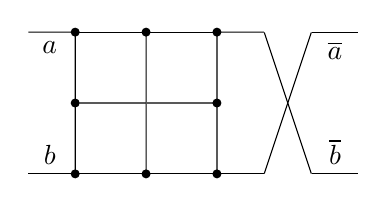
\begin{tikzpicture}[auto, scale=0.3]
	
	\node (bA) [scale=0.03] at (13, 6) {};
    \node (b1) [circle, draw, fill, scale=0.3] at (15, 6) {};
    \node (b2) [circle, draw, fill, scale=0.3] at (18, 6) {};
    \node (b3) [circle, draw, fill, scale=0.3] at (21, 6) {};
    \node (bC) [scale=0.03] at (23, 6) {};
    \node (bDC) [scale=0.03] at (25, 6) {};
    \node (bDCC) [scale=0.03] at (27, 6) {};
        
    \node (b4) [circle, draw, fill, scale=0.3] at (15, 3) {};
    \node (b5) [scale=0.03] at (18, 3) {};
    \node (b6) [circle, draw, fill, scale=0.3] at (21, 3) {};
    
    \node (bB) [scale=0.03] at (13, 0) {};
    \node (b7) [circle, draw, fill, scale=0.3] at (15, 0) {};
    \node (b8) [circle, draw, fill, scale=0.3] at (18, 0) {};
    \node (b9) [circle, draw, fill, scale=0.3] at (21, 0) {};
    \node (bD) [scale=0.03] at (23, 0) {};
    \node (bCD) [scale=0.03] at (25, 0) {};
    \node (bCDD) [scale=0.03] at (27, 0) {};
    
    \path[-]
    (bB) edge node[above] {$b$} (b7)
    (bA) edge node[below] {$a$} (b1)
    (b1) edge (b4)
    (b4) edge (b7)
    (b2) edge (b1)
    (b4) edge (b5)
    (b5) edge (b6)
    (b7) edge (b8)
    (b2) edge (b5)
    (b5) edge (b8)
    (b3) edge (b2)
    (b8) edge (b9)
    (b9) edge (b6)
    (b3) edge (b6)
    (bC) edge (b3)
    (bC) edge (bCD)
    (bCD) edge node[above] {$\overline{b}$} (bCDD)
    (b9) edge (bD)
    (bD) edge (bDC)
    (bDC) edge node[below] {$\overline{a}$} (bDCC);
    
\end{tikzpicture}
